\question \textbf{DP table cell update rules}
  
Dynamic programming (DP) is an algorithm that uses table cells to memorize the sub-solutions of the target solution. DP requires three candidate scores and selects the maximum score among them when updating a cell.

\begin{align*}
H_{i,j}^{(0)} &= H_{i-1,j} - g &(vertical) \\
H_{i,j}^{(1)} &= H_{i,j-1} - g	&(horizontal) \\
H_{i,j}^{(2)} &= H_{i-1,j-1} + R_{a,b} &(diagonal)
\end{align*}

Use the simple scoring scheme below to calcualte $H_{i,j}$ in Table A and B. 

\textbf{Scoring scheme: }\\
\null \quad $R_{ab}$ = 1 for a = b \\ 
\null \quad $R_{ab}$ = 0 for a $\neq$ b \\ 
\null \quad g = 1  

\vspace{0.1 in}

\begin{parts}

%% (a)
\part Table A

\begin{figure}[h]
  \centering
      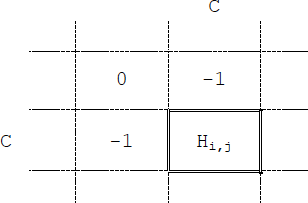
\includegraphics[width=0.325 \textwidth]{fig02/cell_update_1.png}
\end{figure}

\begin{solution}[0.75 in]
1
\end{solution}

%% (b)
\part  Table B

\begin{figure}[!h]
  \centering
      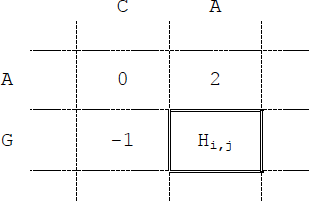
\includegraphics[width=0.325 \textwidth]{fig02/cell_update_2.png}
\end{figure}

\begin{solution}[0.75 in]
1
\end{solution}

\end{parts}

\pagebreak
